\documentclass[10pt,a4paper,twoside]{article}
\usepackage{graphicx}
\usepackage{latexsym,theorem}
\usepackage{isabelle,isabellesym}
\usepackage{pdfsetup} %last one!

\isabellestyle{it}
\urlstyle{rm}

\newcommand{\isasymsup}{\isamath{\sup\,}}


\begin{document}

\pagestyle{headings}
\pagenumbering{arabic}

\title{The Hahn-Banach Theorem \\ for Real Vector Spaces}
\author{Gertrud Bauer}
\maketitle

\begin{abstract}
  The Hahn-Banach Theorem is one of the most fundamental results in functional
  analysis. We present a fully formal proof of two versions of the theorem,
  one for general linear spaces and another for normed spaces.  This
  development is based on simply-typed classical set-theory, as provided by
  Isabelle/HOL.
\end{abstract}


\tableofcontents
\parindent 0pt \parskip 0.5ex

\clearpage
\section{Preface}

This is a fully formal proof of the Hahn-Banach Theorem. It closely follows
the informal presentation given in Heuser's textbook \cite[{\S} 36]{Heuser:1986}.
Another formal proof of the same theorem has been done in Mizar
\cite{Nowak:1993}.  A general overview of the relevance and history of the
Hahn-Banach Theorem is given by Narici and Beckenstein \cite{Narici:1996}.

\medskip The document is structured as follows.  The first part contains
definitions of basic notions of linear algebra: vector spaces, subspaces,
normed spaces, continuous linear-forms, norm of functions and an order on
functions by domain extension.  The second part contains some lemmas about the
supremum (w.r.t.\ the function order) and extension of non-maximal functions.
With these preliminaries, the main proof of the theorem (in its two versions)
is conducted in the third part.  The dependencies of individual theories are
as follows.

\begin{center}
  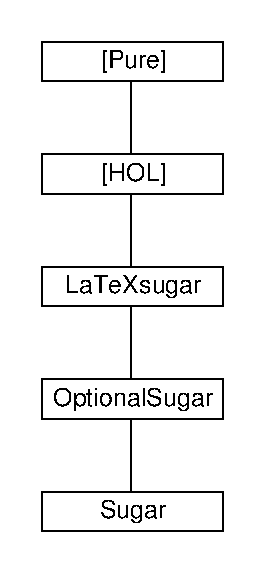
\includegraphics[scale=0.5]{session_graph}  
\end{center}

\clearpage
\part {Basic Notions}

\input{Bounds}
\input{Vector_Space}
\input{Subspace}
\input{Normed_Space}
\input{Linearform}
\input{Function_Order}
\input{Function_Norm}
\input{Zorn_Lemma}

\clearpage
\part {Lemmas for the Proof}

\input{Hahn_Banach_Sup_Lemmas}
\input{Hahn_Banach_Ext_Lemmas}
\input{Hahn_Banach_Lemmas}

\clearpage
\part {The Main Proof}

\input{Hahn_Banach}
\bibliographystyle{abbrv}
\bibliography{root}

\end{document}
